\documentclass[11pt]{article}

\usepackage[normalem]{ulem}
\useunder{\uline}{\ul}{}
\usepackage{setspace}
%modifier la mise en page de l'abstract
\usepackage{abstract}
%police et mise en page (marges) du document
\usepackage[T1]{fontenc}
\usepackage[top=2cm, bottom=2cm, left=2cm, right=2cm]{geometry}
\usepackage{babel}
\usepackage{titling}
\usepackage{blindtext}
\usepackage{amsmath}
\usepackage{amsfonts}
\usepackage{multicol}
\usepackage{fancyvrb}
\usepackage{fancyhdr}
\usepackage{enumitem}
\usepackage{graphicx}
\usepackage{hyperref}
\renewcommand{\labelitemi}{$-$}
\setlength{\headheight}{13.6pt}
%\setlist[itemize]{itemsep=0pt}
\author{}

\begin{document}


\pagestyle{fancy}
\fancyhead{}
\fancyhead[L]{TFE - Création d'une application pour conception et organisation de spectacles}
\fancyhead[R]{D. van Rossum}


\title{\vspace{-1cm}\huge{Requirements}\vspace{-1.7cm}}
\date{}
\maketitle
\thispagestyle{fancy}
\section{Functionalities}
\subsection{For rehearsal organizers}

\subsubsection{Creat a project}
The organizer can create a project by assigning it a name.

\subsubsection{Add people to the project}
The organizer will be able to encode which user are working on the project and add their role(s) (dancer, actor, technician, organizer, etc.), the users will be found based on their email address.

\subsubsection{More than one organiser}
If a person is added with the role organizer, they will have the same right as the organizer who made the project.

\subsubsection{Contact list}
The organizer has access to a list of professionals involved in the project. The contact details for each person should include their full name, profession, role on the project (dancer, actor, technician, etc.) and contact information (email)

\subsubsection{Ability to add someone without an account}
If the organizer adds the email address of someone who does not already have an account, that person will receive an invitation via email to create an account.

\subsubsection{Encode rehearsal needs}
The organizer can encode the specific needs for each rehearsal by selecting which professionals are required for the rehearsal and defining the rehearsal duration. 

\subsubsection{Encode rehearsal order}
The organizer can define an order between the different rehearsal created.

\subsubsection{Computation for suggestions of rehearsal time slots} 
The application will compute a suggestion for optimal rehearsal time slots based on participants' availability. It will analyse the provided availability and propose the best possible times when the maximum number of participants can attend.

\subsubsection{Calendar with the availability of everyone}
The organizer will have access to a calendar that integrates the availability of all participants. It will allow:
\begin{itemize}
    \item Visualization of participants' availability in time slots (available, maybe available, not available).
    \item Automatic suggestions for optimal rehearsal times based on everyone's availability.
    \item Ability to select a proposed time slot or see everyone's availability for other slots.
\end{itemize}

\subsubsection{Notifications if the availability of someone changes}
When a participant modifies their availability and this impacts the rehearsal schedule (time slots not possible anymore or better time slots now possible), the app will:
\begin{itemize}
    \item Send a notification to the organizers, indicating the affected time slots.
    \item Suggest alternatives (new time slots) if necessary.
    \item Allow the organizer to either adjust the schedule or keep the rehearsal without the unavailable participant.
\end{itemize}

\subsection{For rehearsal organizers and participants}

\subsubsection{Create an account}
Each user must create an account by specifying their name, profession, email address, and whether they are a participant or an organizer.

\subsubsection{Authentification}
The application will include an authentication system, allowing users to log in and log out of their account.

\subsubsection{Ability to reject a project}
Users can see the projects they have been added to, with the option to reject the invitation.

\subsubsection{Personal calendar}
Users can access a calendar displaying all of their rehearsals.

\subsubsection{Exprort Calendar}
Users can export their calendar to external systems (e.g., Google Calendar, Outlook).

\subsubsection{Can encode their availability}
Users can specify their availability within the app by selecting a time range and one of the following statuses: 
\begin{itemize} 
    \item Not Available (cannot participate) 
    \item Maybe Available (can participate with some constraints) 
    \item Available (ready to participate) 
\end{itemize}

\subsubsection{Notifications if personal schedule changes}
When a rehearsal is rescheduled and affects a user's agenda, the app will send a notification to that user. This notification will specify:
\begin{itemize}
    \item The nature of the change (time change, location change, addition or cancellation of a rehearsal).
    \item The new information to be taken into account in their calendar.
\end{itemize}

\subsubsection{Notification if schedule of pre-selected participant changes}
A user can select certain participants to monitor their availability. If the availability of these participants changes, the user will receive a notification informing them of the changes.

\subsubsection{RGPD and Data Protection Impact Assessment (DPIA)}
The application will comply with the General Data Protection Regulation (GDPR) regarding the management of personal information and Data Protection Impact Assessment (DPIA).

\subsubsection{European Accessibility Act (EAA)}
The application will comply with the \href{https://eur-lex.europa.eu/legal-content/EN/TXT/?uri=CELEX%3A32019L0882}{European Accessibility Act} (EAA) requirements, ensuring accessibility for people with disabilities in key functionalities.

\section{User scenario}

\begin{enumerate}
    \item Jean creates a project name "Winter Wonderland", for his new show.
    \item Jean adds to the project Lilia as the main dancer. He adds Baptist as the technician. Jean also adds Ryan as a backup dancer.
    \item Jean add two rehearsal, one with Lilia and Ryan and one with Lilia, Baptist and Ryan. He specified that the first one takes 2h30 and the second 4 hours.
    \item Two days latter Jean receives all the availabilities of Lilia, Baptist and Ryan. He selects all the proposed time slots and approve them.
    \item Jean receives a notification saying that Ryan isn't available at the rehearsal time anymore.
    \item Jean decide to keep the rehearsal at the same time and just do it without Ryan.
\end{enumerate}

\newpage
\section{Planning}
%proposez des time slots
\begin{table}[htbp]
    \centering
    \begin{tabular}{| p{9cm} | p{2cm} | p{2.1cm} | p{2cm} |}
    \hline
    \textbf{Task Name} & \textbf{Duration} & \textbf{Start Date} & \textbf{End Date} \\
    \hline
    \textbf{Sprint 0} &&&\\
    \quad Need analysis & 2 weeks & 16-09-2024 & 02-10-2024 \\
    \quad Requirements & 2 weeks & 03-10-2024 & 16-10-2024 \\
    \textbf{Sprint 1} &&&\\
    \quad Authentication & 1 week & 10-10-2024 & 16-10-2024 \\
    \quad Design database schema & 1 week & 17-10-2024 & 23-10-2024 \\
    \quad Create an account & 1 week & 24-10-2024 & 30-10-2024 \\
    \quad Analyse European Accessibility Act (EAA) & 1 week & 24-10-2024 & 30-10-2024 \\
    \quad Test the implemented functionalities & 1 week & 31-10-2024 & 06-11-2024\\
    \textbf{Sprint 2} &&&\\
    \quad Create project & 1 week & 07-11-2024 & 13-11-2024 \\
    \quad Add people to the project & 1 week & 14-11-2024 & 20-11-2024 \\
    \quad If role is organizer becomes an organizer & 1 week & 14-11-2024 & 20-11-2024 \\
    \quad Add someone without an account & 1 week & 21-11-2024 & 27-11-2024 \\
    \quad Test the implemented functionalities & 1 week & 28-11-2024 & 04-12-2024\\
    \textbf{Sprint 3} &&&\\
    \quad Contact list & 1 week & 05-12-2024 & 11-12-2024 \\
    \quad Encode rehearsal needs & 1 week & 12-12-2024 & 18-12-2024 \\
    \quad Encode rehearsal order & 1 week & 03-02-2025 & 05-02-2025 \\
    \quad Test the implemented functionalities & 1 week & 06-02-2025 & 12-02-2025\\
    \textbf{Sprint 4} &&&\\
    \quad Ability to reject a project & 1 week & 13-02-2025 & 19-02-2025 \\
    \quad Encode availability & 1 week & 20-02-2025 & 26-02-2025 \\
    \quad Test the implemented functionalities & 1 week & 27-02-2025 & 05-03-2025\\
    \textbf{Sprint 5} &&&\\
    \quad Computation for suggestions of rehearsal time slots & 2 weeks & 06-03-2025 & 19-03-2025 \\
    \quad Calendar with everyone's availability & 2 weeks & 20-03-2025 & 02-04-2025 \\
    \quad Notify organizers & 1 week & 03-04-2025 & 09-04-2025 \\
    \quad Test the implemented functionalities & 1 week & 10-04-2025 & 16-04-2025\\
    \textbf{Sprint 6} &&&\\
    \quad Personal calendar & 1 week & 17-04-2025 & 23-04-2025 \\
    \quad Export calendar & 1 week & 24-04-2025 & 30-04-2025 \\
    \quad Notify participants & 1 week & 01-05-2025 & 07-05-2025 \\
    \quad Test the implemented functionalities & 1 week & 08-05-2025 & 14-05-2025\\
    \textbf{RGPD and DPIA} & 2 weeks & 15-05-2025 & 28-05-2025 \\
    \textbf{User testing} & 4 weeks & 29-05-2025 & 25-06-2025\\
    \hline
    \end{tabular}
\end{table}

\newpage

\vspace{1cm}
\hspace{-1.5cm}
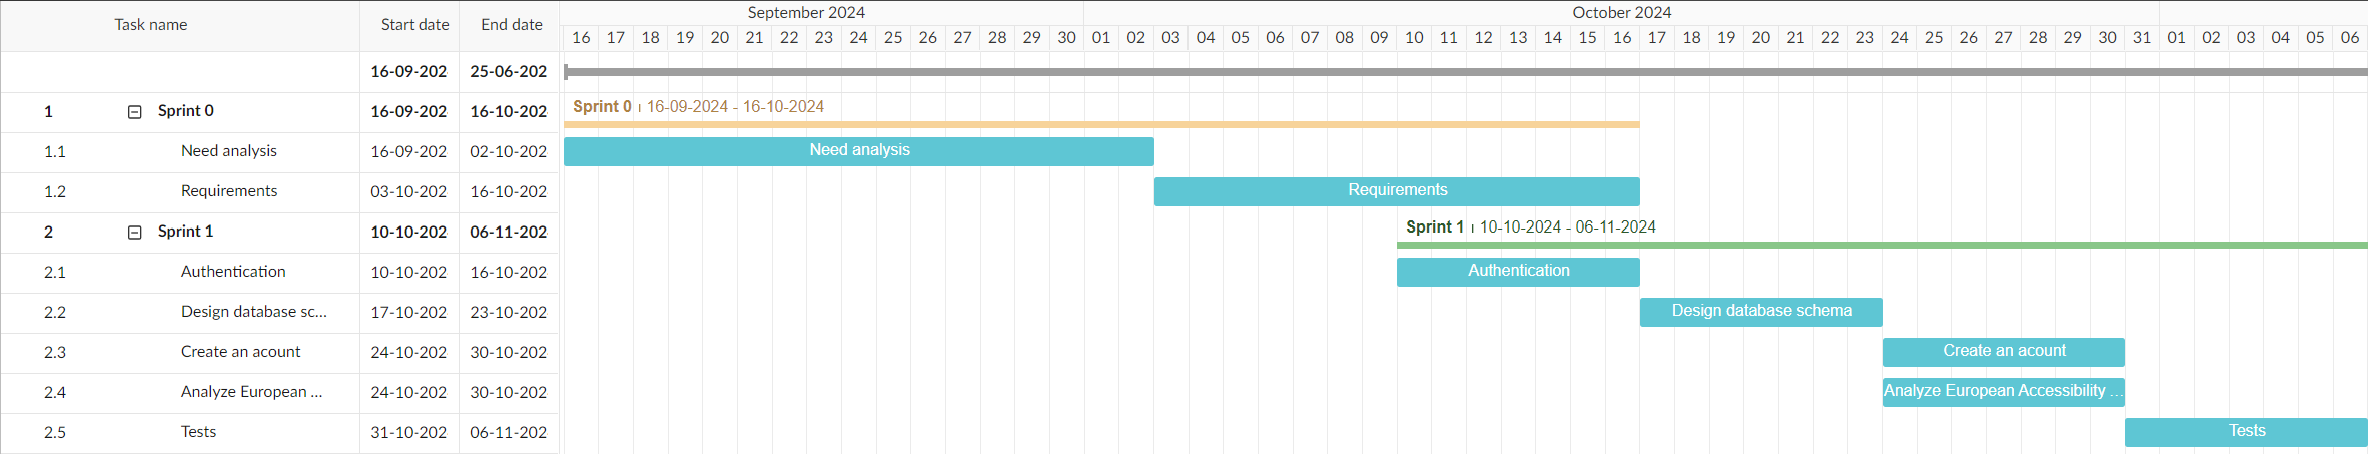
\includegraphics[scale=0.6]{g1.png}

\vspace{1cm}
\hspace{-1.5cm}
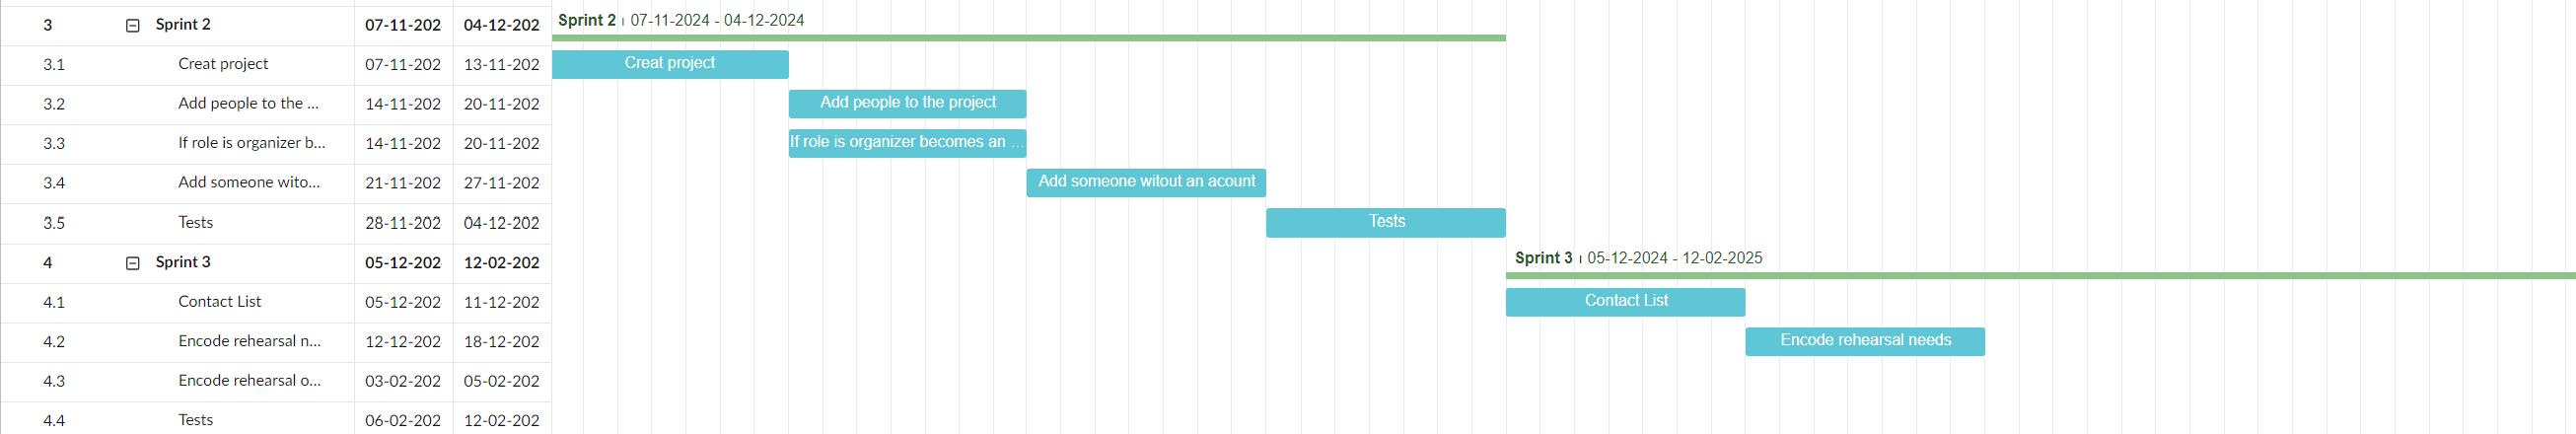
\includegraphics[scale=0.57]{g2.png} 

\vspace{1cm}
\hspace{-1.5cm}
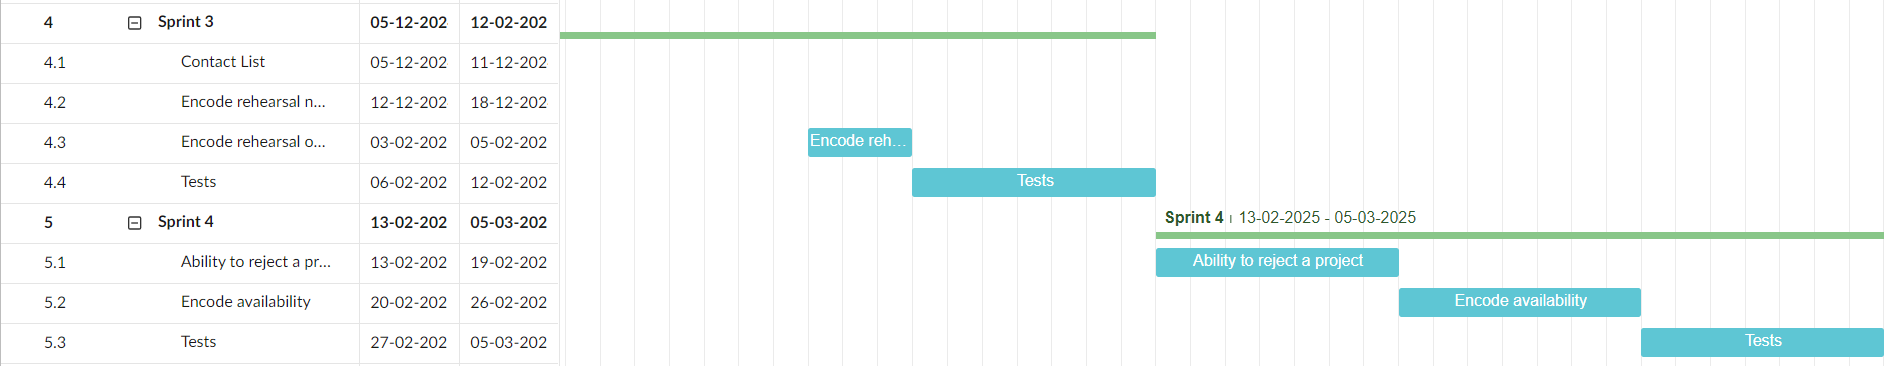
\includegraphics[scale=0.75]{g3.png} 

\vspace{1cm}
\hspace{-1.5cm}
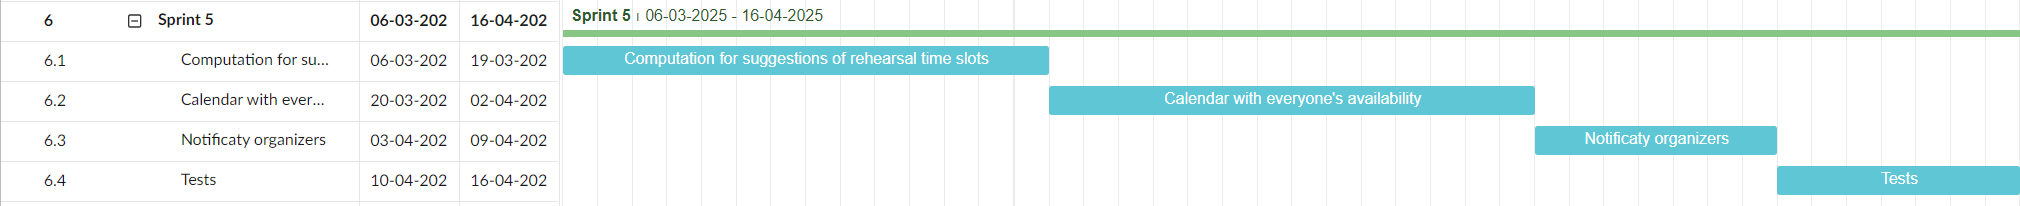
\includegraphics[scale=0.71]{g4.png} 

\vspace{1cm}
\hspace{-1.5cm}
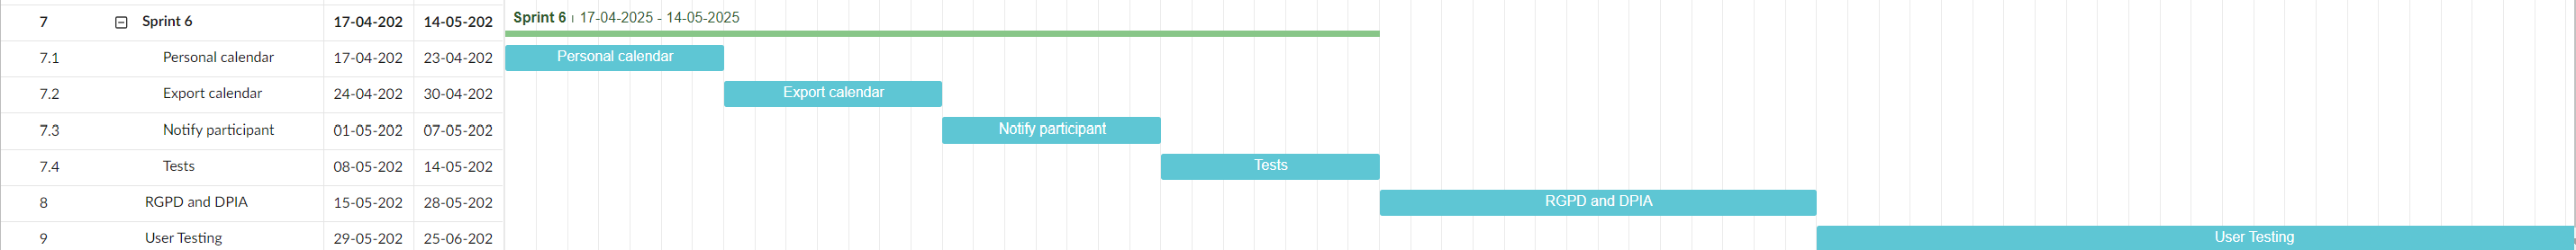
\includegraphics[scale=0.5]{g5.png} 

%\newpage

\vspace{1.5cm}

\section{Activity Diagram}

\begin{figure}[htbp!]
    \centering
    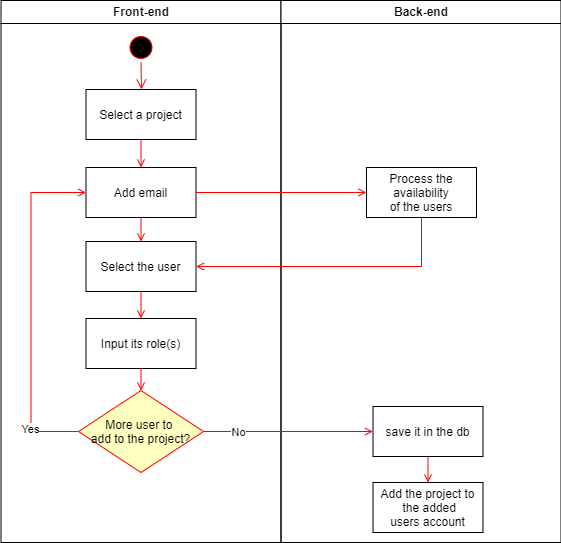
\includegraphics[scale=0.5]{projectinit.drawio.png}
    \caption{Activity diagram, Adding user to a project}
\end{figure}

\begin{figure}[htbp!]
    \centering
    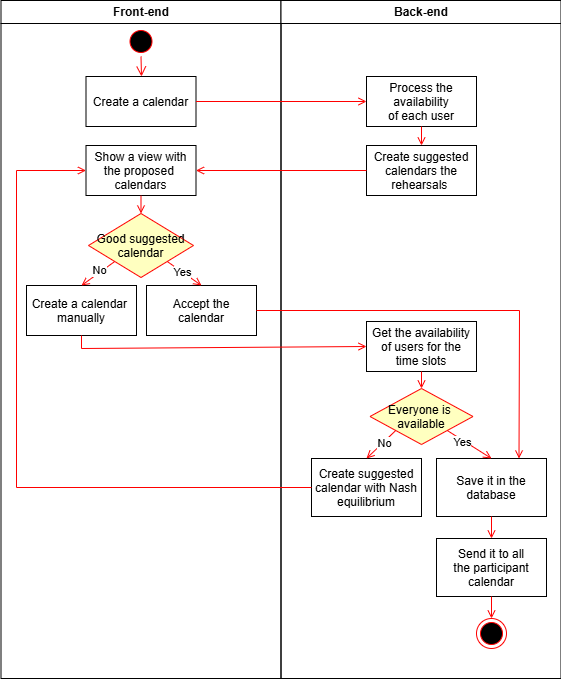
\includegraphics[scale=0.5]{calendarselection.drawio.png}
    \caption{Activity diagram, Calendar with the availability of everyone}
\end{figure}


\end{document}